\documentclass{article}

% Language setting
% Replace `english' with e.g. `spanish' to change the document language
\usepackage[english]{babel}

% Set page size and margins
% Replace `letterpaper' with `a4paper' for UK/EU standard size
\usepackage[letterpaper,top=2cm,bottom=2cm,left=3cm,right=3cm,marginparwidth=1.75cm]{geometry}

% Useful packages
\usepackage{amsmath}
\usepackage[font=small,labelfont=bf]{caption}
\usepackage{graphicx}
\usepackage{microtype}
\usepackage[colorlinks=true, allcolors=blue]{hyperref}

\graphicspath{{figures/}}
\newcommand{\figref}[1]{Fig.~\ref{#1}}

\title{Reset as a Targeting Problem in Recurrent Spiking Networks}
\author{Jack Large, Jasper Mark}

\begin{document}
\maketitle

\begin{abstract}
  A central goal for cultured and engineered neural systems is a reset: a stimulus that returns a trained network to a naive, retrainable state. Whether open-loop electrical stimulation can achieve this, and what its failure would reveal, remains unknown. Using a recurrent spiking network model of a cortical culture in which the synaptic state is observable but, as in wetware, can be reached only through a 64-channel electrode interface, we screened a broad space of spectral, temporal, and spatial stimulation protocols against a behavioral readout validated to track the synaptic memory trace. In a 50-seed replication across six task families, broadband stimulation drove large synaptic and activity perturbations, yet no protocol returned behavior to chance or reduced relearning savings. This dissociation was geometric: moving weights toward the naive state along the training-defined synaptic direction eventually crossed criterion in nearly all seed--task cases, whereas matched random orthogonal displacement never did; surgical ablations further showed that task performance depends on sparse electrode-defined input and target pathways rather than bulk synaptic displacement. For these electrode-association tasks, the learned representation is pathway-specific and aligned to a task-relevant synaptic direction that untargeted stimulation structurally fails to reach. The result reframes reset as a targeting problem and suggests that successful reset may require targeted closed-loop control capable of selectively perturbing task-relevant synaptic subspaces.
\end{abstract}

\section{Methods}

\subsection{Network model}

We simulated a dissociated cortical culture as a spatially embedded recurrent network of leaky integrate-and-fire neurons. Neurons were placed at random positions on a planar field and assigned excitatory or inhibitory identity with fixed probability. Connectivity was distance-biased: each neuron projected to a set of nearby targets drawn with probability decaying exponentially in inter-neuronal distance, supplemented by a sparse population of long-range recurrent connections. Excitatory synapses were plastic under a fixed-sign spike-timing-dependent plasticity rule with separate potentiation and depression time constants, and a slow homeostatic mechanism rescaled excitatory weights toward a target population firing rate. Synaptic signs were fixed at initialization and preserved under all subsequent manipulations, so that no analysis or perturbation could convert an excitatory synapse into an inhibitory one or vice versa. All reported experiments used networks of $10^4$ neurons. The full synaptic weight vector and all spike times were retained for analysis, but neither was accessible to the stimulation or readout pathway.

\subsection{Electrode interface and behavioral task}

The network was actuated and observed only through a simulated 64-channel multielectrode array, mirroring the constraints of a wetware culture. Stimulation entered the network as charge-balanced pulse events delivered to electrode channels, each event driving the subset of neurons nearest that channel. Observation was limited to channel-level multi-unit activity: per-channel spike counts and times pooled over the neurons assigned to each electrode. The learned task was an electrode-to-electrode conditioned association. During training, an input-electrode pulse was paired with a target-electrode pulse at a fixed delay, and native plasticity strengthened the pathway that made the target response follow the input. We studied six task families: single association, pattern discrimination, overlapping shared-target mappings, overlapping shared-input mappings, multi-association mappings, and XOR-like electrode classification. Networks were trained to a behavioral criterion or for a fixed maximum number of repetitions, whichever came first.

\subsection{Behavioral readout and its controls}

The behavioral score was defined as the difference between the response probability on positive (trained) probes and the response probability on negative or cross probes, evaluated with plasticity disabled and averaged over repeated probe presentations from identical cloned states. Before using this score to evaluate reset, we required it to pass two controls. First, the score had to be input-specific: a trained network must respond to the genuine input pulse but not to a matched sham probe. Second, and most stringently, the score had to be weight-dependent: overwriting the trained synaptic weights with the pre-training (naive) weights, while leaving every other state variable intact, had to return the score to chance. This naive-weight overwrite served throughout as the privileged positive control --- the one manipulation guaranteed to remove the learned synaptic trace, and the ceiling against which stimulation was compared.

\subsection{Paired-clone reset assay}

Reset was evaluated by a within-state paired comparison. For each network seed and task, we trained once to criterion and then cloned the entire trained state, including synaptic weights, membrane variables, plasticity traces, and homeostatic variables. From this clone we ran two matched branches: a reset branch, which received a candidate stimulation protocol, and a no-reset branch, which received an equal duration of plasticity-on rest. Behavioral score, synaptic state, channel activity, and subsequent relearning were measured on both branches, so that every reported effect of stimulation is a difference between two branches descended from the same trained state.

\subsection{Stimulation protocol space}

Candidate reset protocols were drawn from a coarse grid spanning three actuator axes expressible through the electrode interface: the temporal color of the stimulation (spectral slope of event timing, from blue through white to red/brown), the schedule (static, alternating-color, epoch--pause, chirp, and gated-burst structures), and the spatial pattern across channels (shared, independent, correlated, or phase-shifted). Stimulation current, pulse width, duration, and pulse count were tracked as cost variables. The grid was a screen of the reachable actuator space rather than an optimization, and protocols were expressed as electrode pulse trains rather than as direct current injection into individual neurons.

\subsection{Outcome measures: apparent, mechanistic, and functional reset}

We distinguished three operationally separate senses of reset. Apparent reset was a reduction of the post-stimulation behavioral score relative to the matched no-reset branch. Mechanistic reset was movement of the synaptic weight vector back toward the naive state; we quantified both the displacement magnitude relative to the no-reset branch and the signed projection of that displacement onto the training-defined synaptic axis, defined as the difference between the trained and naive weight vectors. This axis is available only in simulation, where the full weight state and the pre-training state are known, and was used for mechanistic interpretation rather than as a biologically observable control signal. Functional reset was a reduction in relearning savings, defined as one minus the ratio of relearning repetitions to initial-learning repetitions, so that a protocol that left no savings would require as many repetitions to retrain as to train initially. A protocol counted as a genuine reset only if it improved all three measures while leaving the network able to relearn.

\subsection{Memory-geometry analyses}

To localize the learned trace in weight space, we performed two analyses on trained networks, exploiting the fact that the synaptic state is observable in the model even though it is hidden from the actuator. First, we measured the breaking point along the training-defined memory axis by interpolating the weight vector between the trained and naive states, $W(\alpha) = (1 - \alpha)\,W_{\mathrm{trained}} + \alpha\,W_{\mathrm{naive}}$, and reading the behavioral score as a function of $\alpha$; the breaking point $\alpha^{*}$ was the smallest fraction of the way to naive at which the score fell below criterion. As a control we displaced the weights by the same magnitude along a random direction orthogonal to the training-defined axis, which asks whether performance degrades with the magnitude or the direction of weight change. Second, we performed surgical ablations against the validated readout, zeroing or scrambling defined synapse sets --- the input-to-target pathway, all edges incoming to target-electrode neurons, all edges outgoing from input-electrode neurons, a magnitude-preserving shuffle, and a magnitude-matched random displacement --- to test whether these electrode-association tasks are stored in a localized, low-dimensional set of connections or distributed across the network.

\subsection{Statistics and reproducibility}

The independent experiment was the network seed within task. The reset screen was replicated across 50 network seeds per task and 60 protocols per task; reported screen summaries use mean, standard deviation, and 95\% confidence intervals across protocol--seed trials or across seeds where stated. Memory-geometry interpolation and surgical ablation analyses were run across 50 network seeds per task for the six-task suite; dimensionality summaries use a fixed channel-pair representation of training-induced weight changes so that seed-wise random graphs can be compared. Reset effects were evaluated as paired differences between the reset and no-reset branches of a common clone, and these paired score differences are the behavioral effect sizes used throughout. Behavioral scores were averaged over repeated plasticity-off probe presentations. All networks, protocols, and analyses were generated from fixed random seeds and are fully reproducible from the recorded run configuration.

\section{Results}

\subsection{Validation of the behavioral readout}

Networks of $10^{4}$ neurons learned electrode-to-electrode associations to criterion within tens of training repetitions. Before using behavior to evaluate reset, we required the readout to pass two controls. The score was input-specific, distinguishing genuine input pulses from matched shams only after training, and it was weight-dependent: overwriting the trained weights with the pre-training weights while leaving all other state intact returned the score to chance (\figref{fig:task-assay}). This naive-weight overwrite --- the one manipulation guaranteed to remove the synaptic trace --- served throughout as the privileged positive control and the ceiling against which stimulation was compared.

\begin{figure}[t]
  \centering
  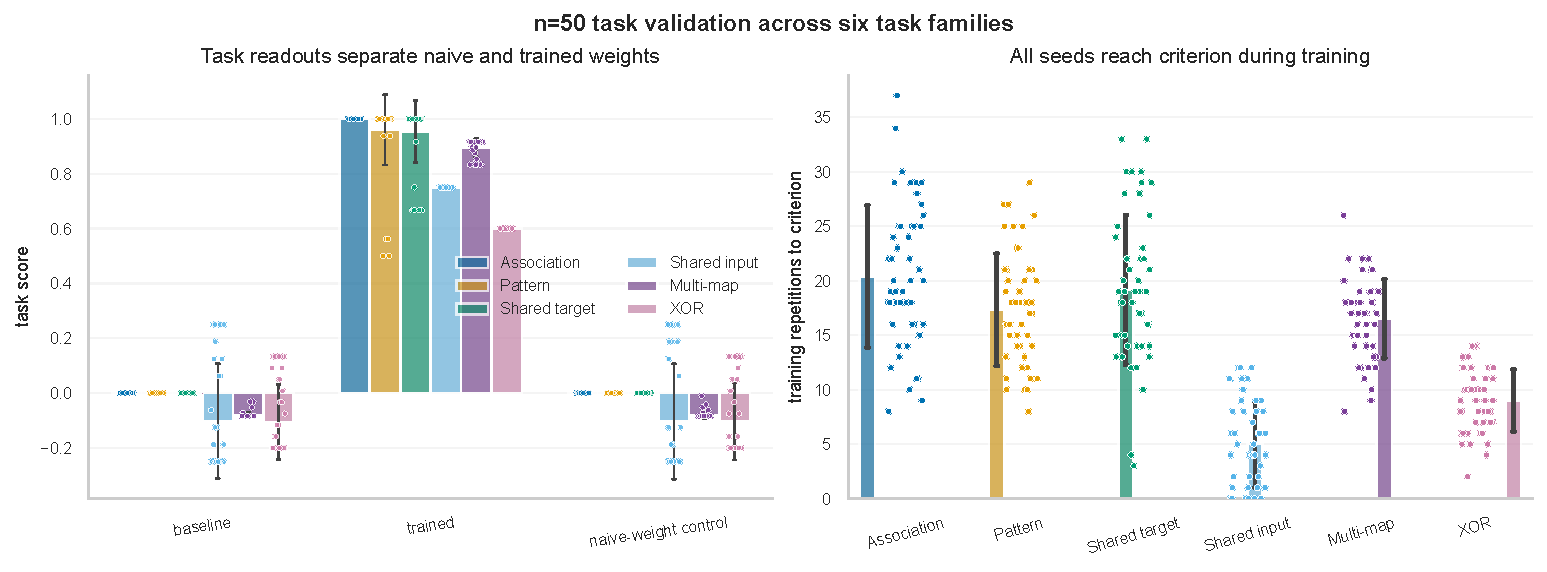
\includegraphics[width=\linewidth]{fig1_task_validation.pdf}
  \caption{\textbf{Validated task assay before reset.}
  \textbf{A,} Across six task families, the behavioral readout separates trained networks from baseline and from the naive-weight control, showing that the measured task score depends on the learned synaptic weights.
  \textbf{B,} All 50 network seeds in each task family reached criterion during training.
  Points denote network seeds; bars show the mean with seed-wise spread.}
  \label{fig:task-assay}
\end{figure}

\subsection{Perturbation without reset}

Across the 50-seed, six-task coarse protocol grid, no stimulation branch met the forgetting criterion in any task. The strongest dents were concentrated in the 50~$\mu$A chirp protocols: the best mean forgetting scores were 0.125 for association, 0.528 for pattern discrimination, 0.372 for shared-target mappings, 0.094 for shared-input mappings, 0.245 for multi-map associations, and 0.075 for XOR. Even in the most affected tasks, post-reset scores remained above criterion, and relearning reached criterion in all cases. Relearning savings remained at ceiling for five tasks and at 0.8 for shared-input mappings, indicating preserved functional memory rather than genuine reset.

\begin{figure}[t]
  \centering
  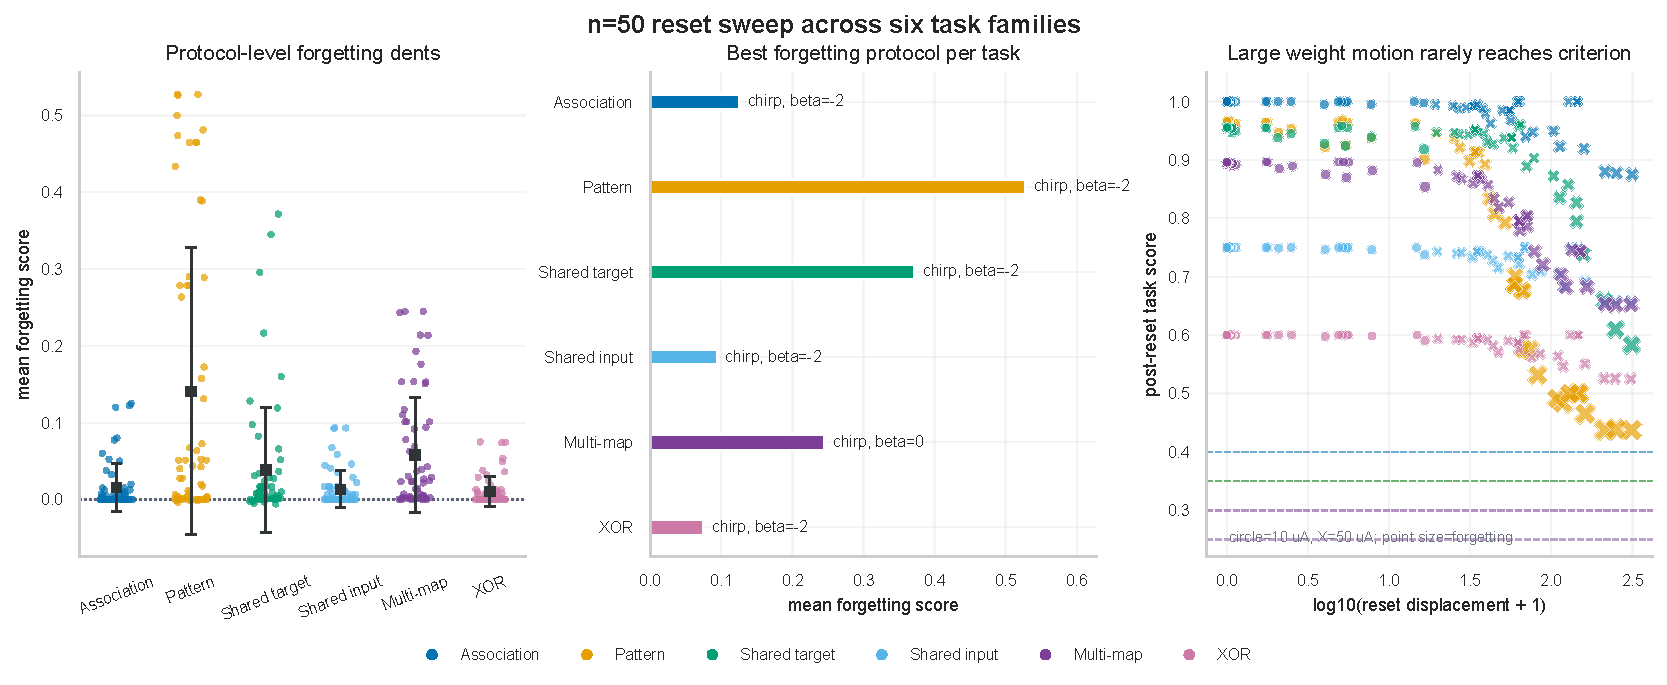
\includegraphics[width=\linewidth]{fig2_reset_sweep_summary.pdf}
  \caption{\textbf{The 50-seed reset sweep does not produce genuine reset.}
  \textbf{A,} Protocol-level mean forgetting dents across six task families.
  \textbf{B,} The strongest protocol in each task remained above the task-specific forgetting criterion.
  \textbf{C,} Large reset-induced recurrent weight displacement did not reliably return behavior to chance; dashed lines mark task criteria.}
  \label{fig:protocol-screen}
\end{figure}

\subsection{Direction versus magnitude of weight change}

Interpolating the weight vector from the trained toward the naive state revealed direction-specific, but not tiny, breaking points. Across 50 seeds per task, the mean axis breaking point ranged from $\alpha^{*}=0.81$ to $0.85$ for association, pattern, shared-target, multi-map, and XOR tasks, and was later for shared-input mappings ($\alpha^{*}=0.94$ among seeds that crossed criterion). In contrast, matched random orthogonal displacement never crossed criterion in any task.

\begin{figure}[t]
  \centering
  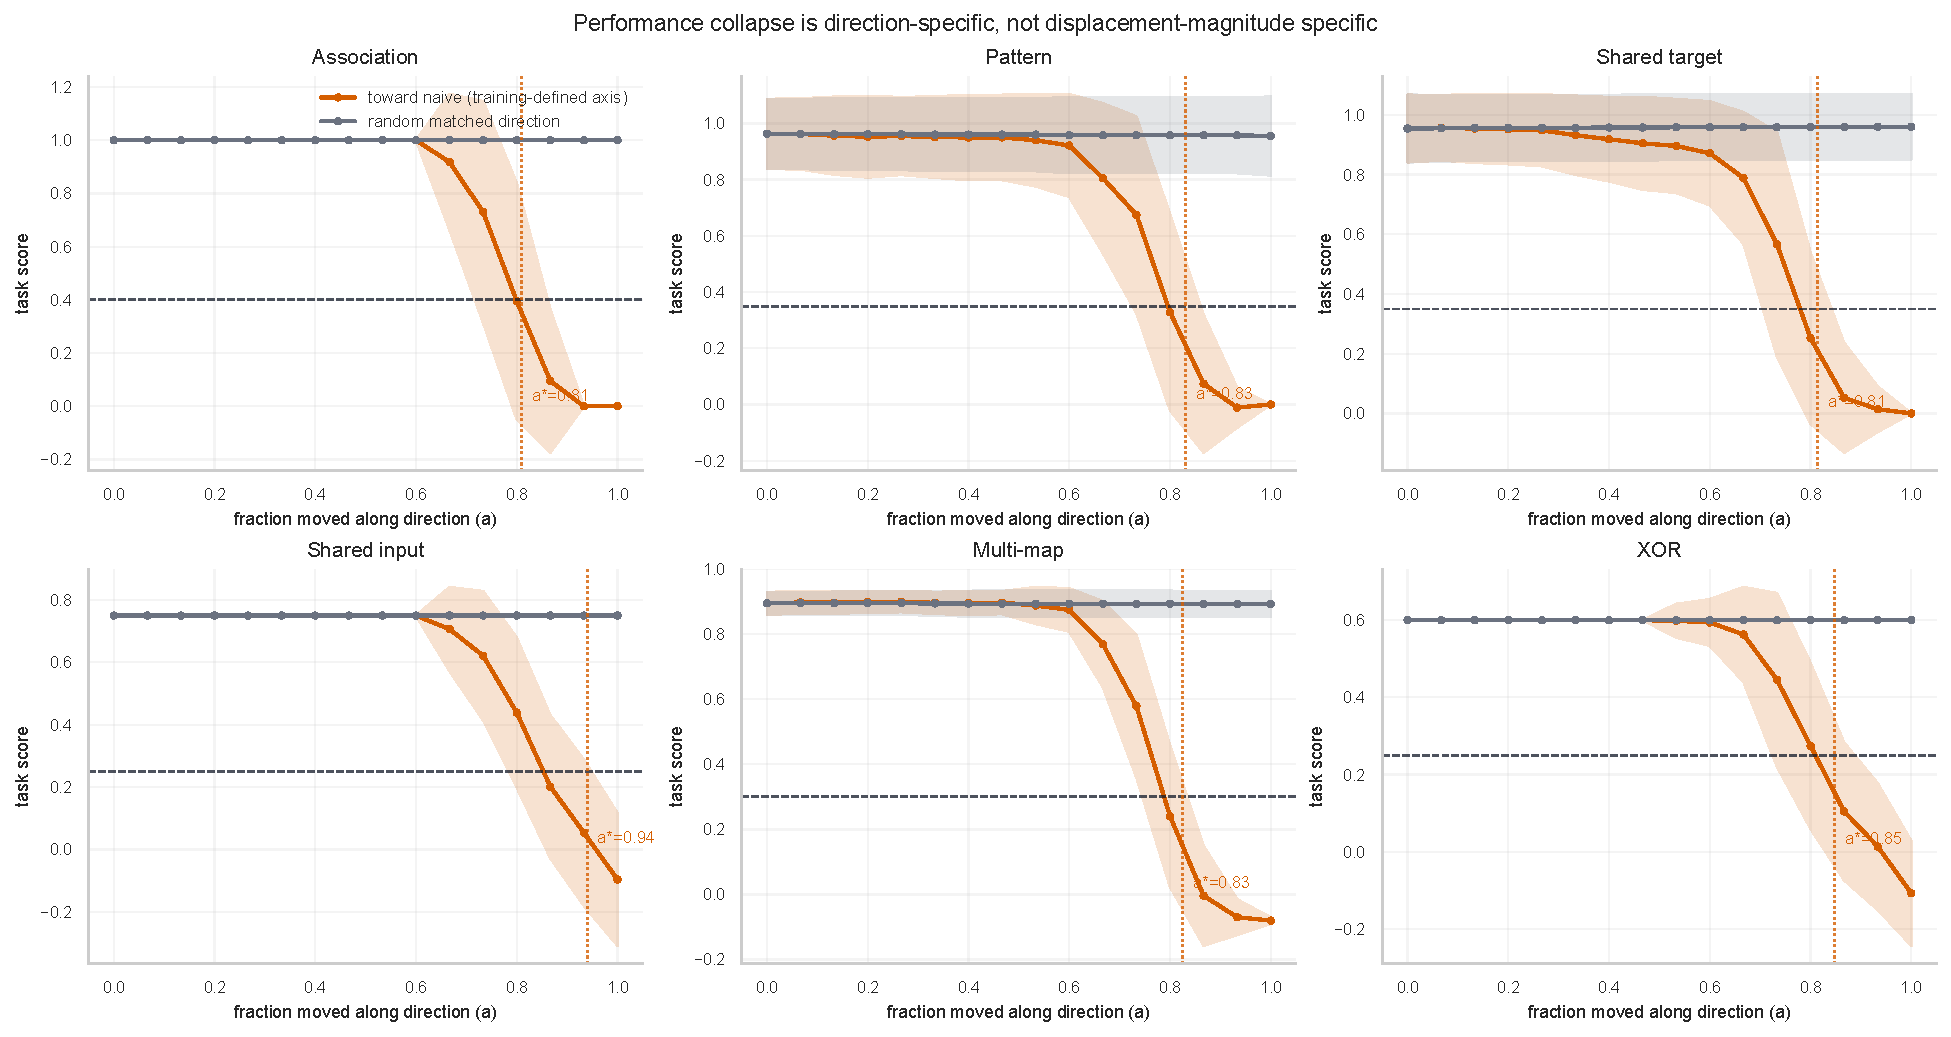
\includegraphics[width=\linewidth]{fig3_breaking_point.pdf}
  \caption{\textbf{Task performance is direction-specific rather than displacement-magnitude specific.}
  Moving weights toward the naive state along the training-defined synaptic direction eventually collapses performance, whereas matched random orthogonal displacement preserves task scores.
  Dashed horizontal lines mark criterion and dotted vertical lines mark the axis breaking point.
  Lines show seed means and shaded bands show seed-wise spread across 50 networks per task.}
  \label{fig:breaking-point}
\end{figure}

\subsection{Localization of the memory trace}

Surgical ablations against the validated readout localized task dependence to electrode-defined input and target pathways rather than to bulk recurrent weight magnitude. Zeroing all outgoing edges from task input electrodes or all incoming edges to task target electrodes abolished or strongly reduced performance across the six tasks, while matched random displacements of comparable norm left performance near trained levels.

\begin{figure}[t]
  \centering
  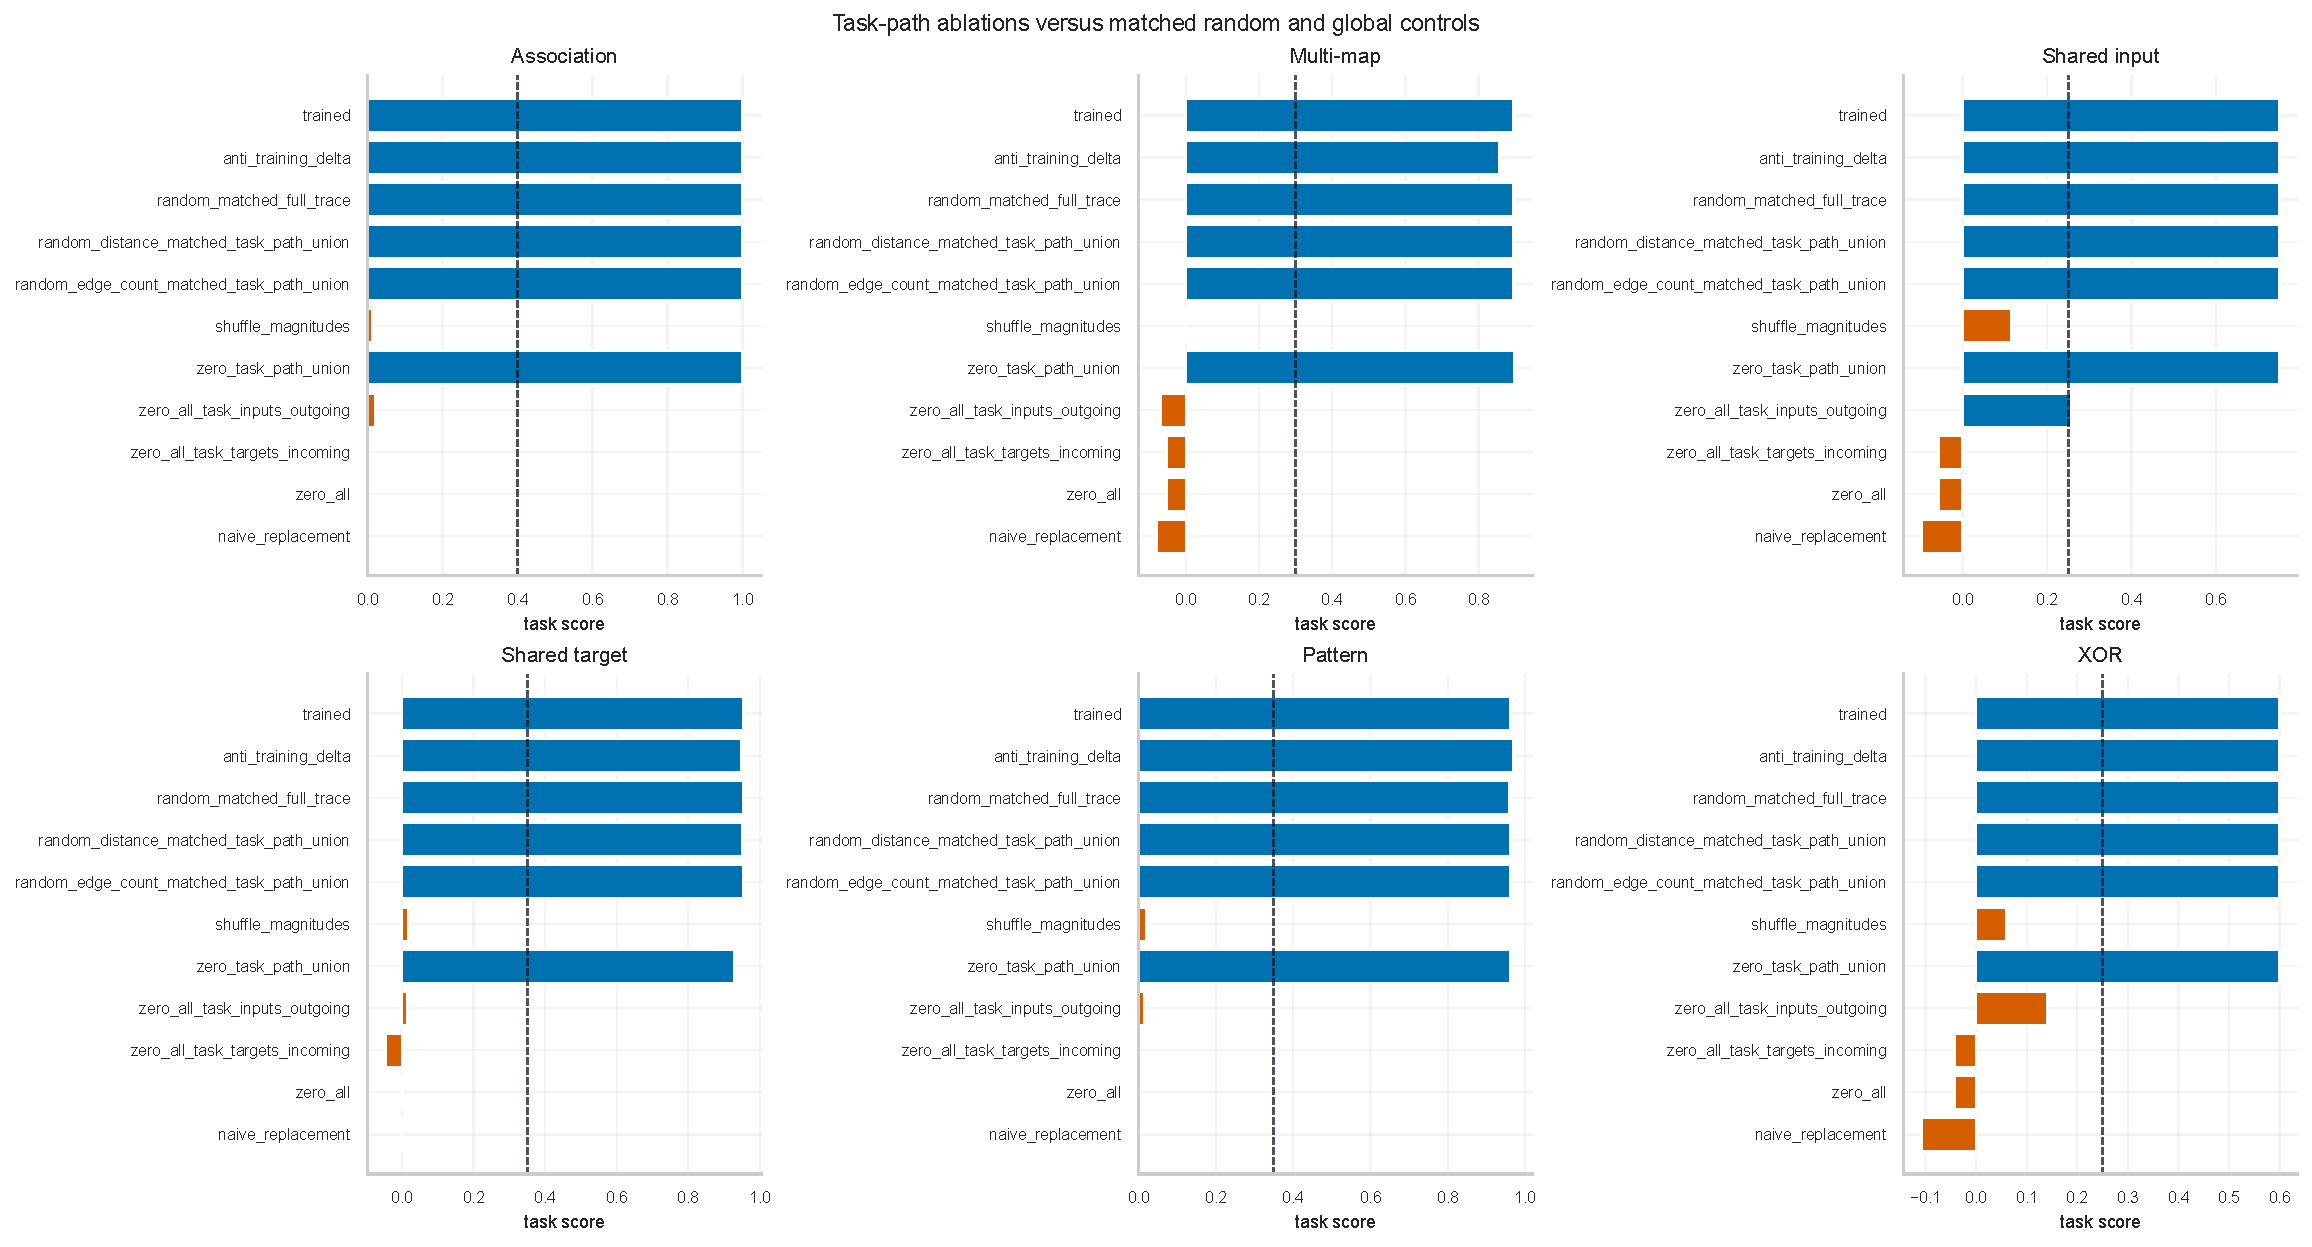
\includegraphics[width=\linewidth]{fig4_ablations.pdf}
  \caption{\textbf{The learned association is pathway-specific.}
  Targeted perturbations to task input and target electrode pathways abolish or strongly reduce performance, while matched random controls and movement away from the training direction leave behavior near the trained state.
  Dashed lines mark task criteria; bars show mean score across 50 network seeds per task.}
  \label{fig:ablations}
\end{figure}

\subsection{A geometric account of reset failure}

Together these results explain why open-loop stimulation suppresses behavior without erasing memory. In these electrode-association tasks, the learned trace has a task-relevant direction that is selectively accessible in simulation but largely missed by open-loop stimulation; performance is much more sensitive to movement toward the naive state along this direction than to matched off-axis displacement. Untargeted stimulation, however large, is delivered through an electrode interface blind to this subspace and so lands almost entirely orthogonal to it. Reset is therefore not only a question of stimulation strength but also of targeting, suggesting that successful reset may require closed-loop control capable of selectively perturbing task-relevant synaptic subspaces.

\subsection{Limitations and biological scope}

The present work should be interpreted as a mechanistic study in a simplified recurrent spiking model rather than a direct model of cultured cortical networks. The model uses leaky integrate-and-fire neurons, pair-based spike-timing-dependent plasticity, and homeostatic scaling; it does not include conductance-based cellular dynamics, heterogeneous cell classes beyond excitatory/inhibitory identity, experimentally measured connectivity distributions, or the full biophysics of dissociated cultures. Accordingly, the biological claim is limited: the simulations show that an electrode-constrained recurrent SNN can preserve a learned association under large open-loop perturbations when those perturbations miss the task-relevant synaptic direction. Whether the same geometry appears in CL1 cultures must be tested with closed-loop wetware experiments and richer model variants.

Two additional limitations follow from the task and analysis design. First, the task families are electrode-association-like, so sparse pathway-specific storage may partly reflect the input-to-target structure of the task. We therefore frame the localization result as evidence for sparse, pathway-specific representations in these electrode-association tasks, not as a general claim that all recurrent SNN memories are sparse. Second, the memory axis is a privileged simulation-only quantity, $W_{\mathrm{trained}} - W_{\mathrm{naive}}$, available because the model exposes the full trained and naive weight states. It is useful for mechanistic interpretation, but it is not an observable biological control variable. Future work should estimate task-relevant subspaces from observable trajectories, for example by PCA or SVD of training-induced weight changes, participation-ratio analyses, and comparisons between variance explained by the training-defined axis and orthogonal axes. The 50-seed reset, interpolation, ablation, and channel-level dimensionality analyses show that the open-loop reset failure and direction-specific geometry are robust across additional network realizations. However, the relevant axis remains a privileged simulation-only quantity, and the task family remains electrode-association-like; stronger claims about biological memory manifolds require observable trajectory-based estimates and wetware validation.

\end{document}
